\documentclass[a4paper, 12pt]{article}
\usepackage[brazil]{babel}
\usepackage[utf8]{inputenc}
\usepackage{indentfirst}
\usepackage{amsmath}
\usepackage{amsthm}
\usepackage{graphicx}
\usepackage{float}
\usepackage[table]{xcolor} % Para colorir as linhas da tabela
\usepackage{array}
\usepackage[font=footnotesize,labelfont=bf]{caption}
\usepackage{geometry}
\usepackage{listings}
\usepackage{subcaption}
\usepackage{xcolor}
\usepackage{float}
\usepackage[skins,xparse,breakable]{tcolorbox}
\usepackage{longtable}
\usepackage{minted}
\usepackage{fancyhdr}
\usepackage[colorlinks=true, allcolors=black]{hyperref}
\usepackage{lastpage}
\usepackage{titlesec} % Para personalizar a formatação das seções

\geometry{a4paper, left=2cm, right=2cm, top=3cm, bottom=2cm}
\definecolor{LightSeaGreen}{rgb}{0.1255, 0.6980, 0.6667}
\definecolor{cinza}{rgb}{0.498, 0.498, 0.498}
\definecolor{whitesmoke}{rgb}{0.96, 0.96, 0.96}

% Redefine o contador de subseções para usar letras
\renewcommand{\thesubsection}{\alph{subsection})}

% Remove a numeração da seção
\renewcommand{\thesection}{}

\makeatletter
\renewcommand*\l@section[2]{%
  \ifnum \c@tocdepth >\z@
    \addpenalty\@secpenalty
    \addvspace{1.0em \@plus\p@}%
    \setlength\@tempdima{0.5em}%
    \begingroup
      \parindent \z@ \rightskip \@pnumwidth
      \parfillskip -\@pnumwidth
      \leavevmode \bfseries % Coloca o título em negrito
      \advance\leftskip\@tempdima
      \hskip -\leftskip
      #1\nobreak\hfil \nobreak\hb@xt@\@pnumwidth{\hss #2}\par
    \endgroup
  \fi
}
\makeatother

% Remove o recuo das seções no documento principal
\titleformat{\section} % Comando para formatar seções
  {\normalfont\Large\bfseries} % Formato do título (negrito e grande)
  {} % Número da seção (vazio, pois não queremos exibir)
  {0em} % Recuo antes do título (0em para remover o recuo)
  {} % Código antes do título (nada adicional)

% Configurações de cabeçalho e rodapé
\pagestyle{fancy}
\fancyhf{}
\fancyhead[L]{\footnotesize{Laboratório de Sistemas Digitais - ENE0040}}
\fancyhead[R]{\footnotesize{2025/1 - Turma 07}}
\fancyfoot[R]{\footnotesize{Página \ \thepage \ de \pageref{LastPage}}}
\fancyfoot[L]{\footnotesize{Relatório do Experimento 1}}

% Adiciona uma linha preta acima do rodapé
\renewcommand{\footrulewidth}{0.4pt} % Espessura da linha
\renewcommand{\footrule}{\vbox to 0pt{\hrule width \textwidth height \footrulewidth \vss}} % Desenha a linha

% Novo Comando para chamar a capa
\newcommand{\capa}{
    \begin{titlepage}
        \begin{center}
            {\large \textbf{ENE0040 - Laboratório de Sistemas Digitais - Turma 07}} \\
            \vspace{3cm}
            {\Huge \textbf{Relatório do Experimento 1}} \\[1em]
            {\large \textbf{Autor:} Henrique Morcelles Salum} \\[0.5em]
            {\large \textbf{Matrícula:} 232003008} \\
            \vfill
            {\Large \textbf{Universidade de Brasília - UnB}} \\[0.75em]
            {\large \textbf{Departamento de Engenharia Elétrica - ENE}} \\
        \end{center}
    \end{titlepage}
}

\begin{document}

\capa

% Sumário
\newpage
\tableofcontents
\newpage

\section{Questão 1}
\paragraph{}
As portas lógicas AND, OR e NOT implementam, respectivamente, as funções booleanas AND, OR e NOT, que seguem, também, respectivamente, as tabelas-verdade a seguir:

\begin{table}[H]
    \centering
    \begin{tabular}{|c|c|c|}
        \hline
        \rowcolor{black}
        \textcolor{white}{$A$} & \textcolor{white}{$B$} & \textcolor{white}{$A \land B$} \\ \hline
        0 & 0 & 0 \\ \hline
        \rowcolor{lightgray}
        0 & 1 & 0 \\ \hline
        1 & 0 & 0 \\ \hline
        \rowcolor{lightgray}
        1 & 1 & 1 \\ \hline
    \end{tabular}
    \caption{Tabela-verdade da função booleana AND}
\end{table}

\begin{table}[H]
    \centering
    \begin{tabular}{|c|c|c|}
        \hline
        \rowcolor{black}
        \textcolor{white}{$A$} & \textcolor{white}{$B$} & \textcolor{white}{$A \lor B$} \\ \hline
        0 & 0 & 0 \\ \hline
        \rowcolor{lightgray}
        0 & 1 & 1 \\ \hline
        1 & 0 & 1 \\ \hline
        \rowcolor{lightgray}
        1 & 1 & 1 \\ \hline
    \end{tabular}
    \caption{Tabela-verdade da função booleana OR}
\end{table}

\begin{table}[H]
    \centering
    \begin{tabular}{|c|c|}
        \hline
        \rowcolor{black}
        \textcolor{white}{$A$} & \textcolor{white}{$\neg A$} \\ \hline
        0 & 1 \\ \hline
        \rowcolor{lightgray}
        1 & 0 \\ \hline
    \end{tabular}
    \caption{Tabela-verdade da função booleana NOT}
\end{table}

\subsection{Implementar uma porta AND usando somente portas OR e NOT}
\paragraph{}
Do Primeiro Teorema de De Morgan obtemos o seguinte resultado:

\[
\overline{A \cdot B} = \overline{A} + \overline{B}
\]
\[
\Rightarrow A \cdot B = \overline{\overline{A} + \overline{B}}.
\]

\noindent Utilizando a notação da Lógica Proposicional, temos:

\[
A \land B = \lnot (\lnot A \lor \lnot B),
\]
ou seja, o AND entre dois bits é o mesmo que o inverso (NOT) do OR entre os inversos desses bits. A implementação desse circuito no Logisim é como segue:

\begin{figure}[H]
    \centering
    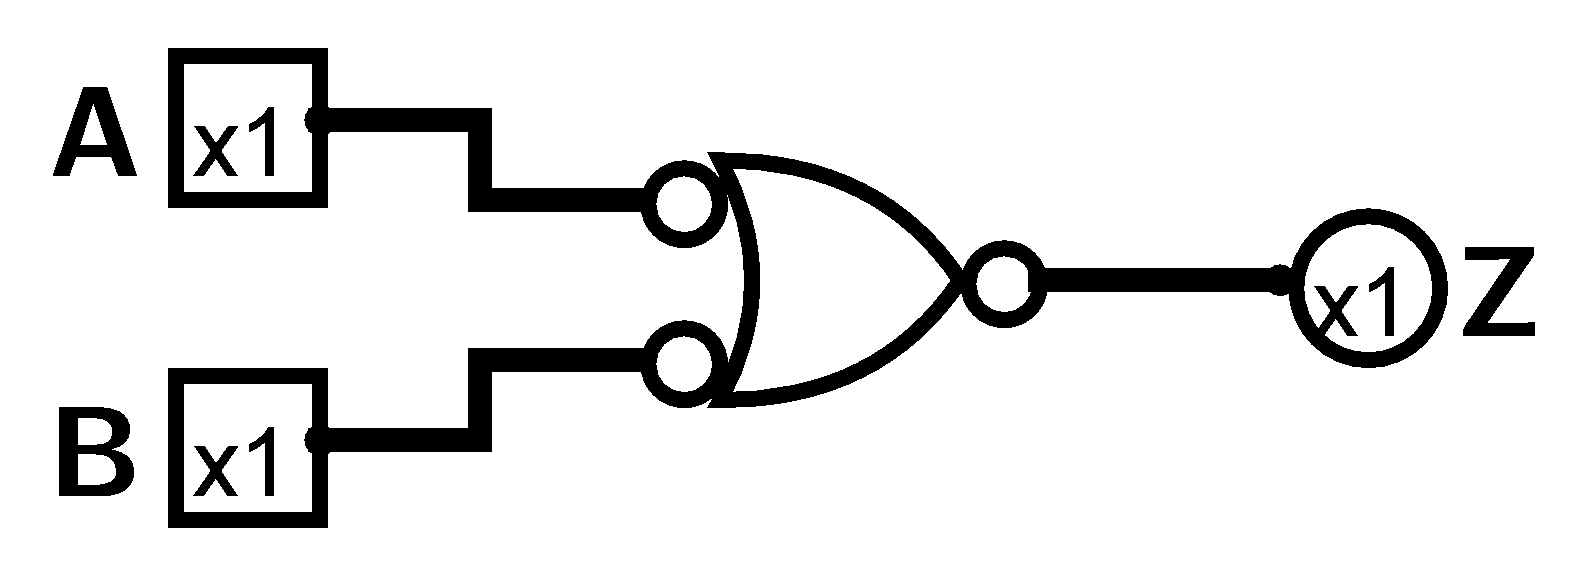
\includegraphics[width=0.3\textwidth]{Imagens/circ1a.png}
    \caption{AND implementado apenas com OR e NOT}
\end{figure}

\begin{figure}[H]
    \centering
    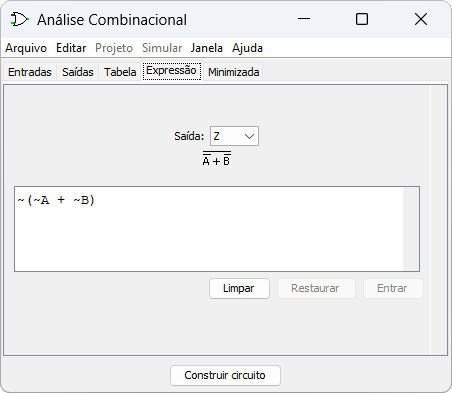
\includegraphics[width=0.4\textwidth]{Imagens/exprQ1a.png}
    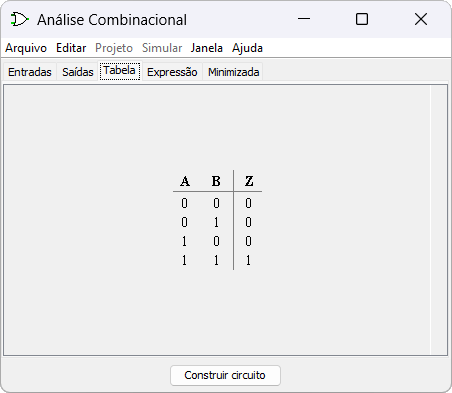
\includegraphics[width=0.4\textwidth]{Imagens/tabQ1a.png} \\
    \caption{Expressão e tabela-verdade gerados pelo Logisim para o circuito da figura 2}
\end{figure}

\subsection{Implementar uma porta OR usando somente portas AND e NOT}
\paragraph{}
Do Segundo Teorema de De Morgan obtemos o seguinte resultado:

\[
\overline{A + B} = \overline{A} \cdot \overline{B}
\]
\[
\Rightarrow A + B = \overline{\overline{A} \cdot \overline{B}}.
\]

\noindent Utilizando a notação da Lógica Proposicional, temos:

\[
A \lor B = \lnot (\lnot A \land \lnot B),
\]

\noindent isto é, o OR entre dois bits é o mesmo que o inverso do AND entre os inversos dos dois bits. A implementação desse circuito no Logisim é como segue:

\begin{figure}[H]
    \centering
    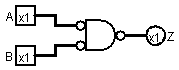
\includegraphics[width=0.3\textwidth]{Imagens/circ1b.png}
    \caption{OR implementado apenas com AND e NOT}
\end{figure}

\begin{figure}[H]
    \centering
    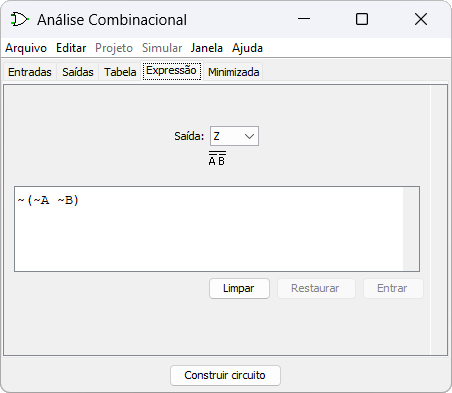
\includegraphics[width=0.4\textwidth]{Imagens/exprQ1b.png}
    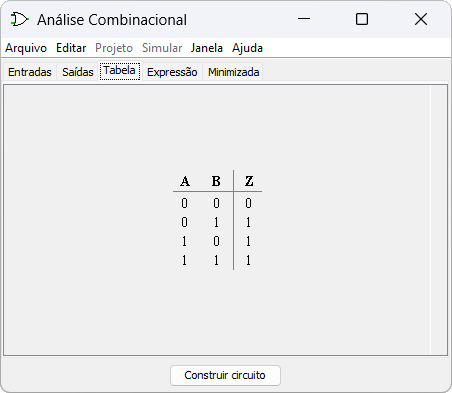
\includegraphics[width=0.4\textwidth]{Imagens/tabQ1b.png} \\
    \caption{Expressão e tabela-verdade gerados pelo Logisim para o circuito da figura 3}
\end{figure}

\section{Questão 2}
\paragraph{}
Nessa questão, implementamos um somador completo. Um somador completo é um circuito lógico combinacional que realiza a soma de três bits: dois bits de entrada, $A$ e $B$, e um bit adicional, $C$ (tipicamente chamado de $C_{in}$, carry-in), que representa o "vai-um" (carry-out) de uma operação anterior. Ele gera duas saídas: $S$, o resultado da soma dos três bits, e $T$ (tipicamente chamado de $C_{out}$, carry-out), o "vai-um" que pode ser gerado por essa soma.
\paragraph{}
As saídas do somador completo, $T$ e $S$, podem ser implementadas, respectivamente, pelas funções booleanas
\[T = AB + AC + BC\] e \[S = \overline{A} \ \overline{B} \ C + \overline{A} \ B \ \overline{C} + A \ \overline{B} \ \overline{C} + A \ B \ C = A \oplus B \oplus C.\] A tabela-verdade a seguir explicita a relação entrada-saída dessas duas funções.

\begin{table}[H]
    \centering
    \begin{tabular}{|c|c|c|c|c|}
        \hline
        \rowcolor{black}
        \multicolumn{3}{|c|}{\textbf{\textcolor{white}{Entradas}}} & \multicolumn{2}{|c|}{\textbf{\textcolor{white}{Saídas}}} \\ \hline
        \rowcolor{black}
        \textcolor{white}{$A$} & \textcolor{white}{$B$} & \textcolor{white}{$C$} & \textcolor{white}{$T$} & \textcolor{white}{$S$} \\ \hline
        0 & 0 & 0 & 0 & 0 \\ \hline
        \rowcolor{lightgray}
        0 & 0 & 1 & 0 & 1 \\ \hline
        0 & 1 & 0 & 0 & 1 \\ \hline
        \rowcolor{lightgray}
        0 & 1 & 1 & 1 & 0 \\ \hline
        1 & 0 & 0 & 0 & 1 \\ \hline
        \rowcolor{lightgray}
        1 & 0 & 1 & 1 & 0 \\ \hline
        1 & 1 & 0 & 1 & 0 \\ \hline
        \rowcolor{lightgray}
        1 & 1 & 1 & 1 & 1 \\ \hline
    \end{tabular}
    \caption{Tabela-verdade das funções $T$ e $S$}
\end{table}

\subsection{Implementar a função T utilizando somente AND e OR}
\paragraph{}
A implementação dessa função é bastante direta: onde na expressão há multiplicação, utilizamos a porta AND e onde há soma, a porta OR. O circuito é o que segue.

\begin{figure}[H]
    \centering
    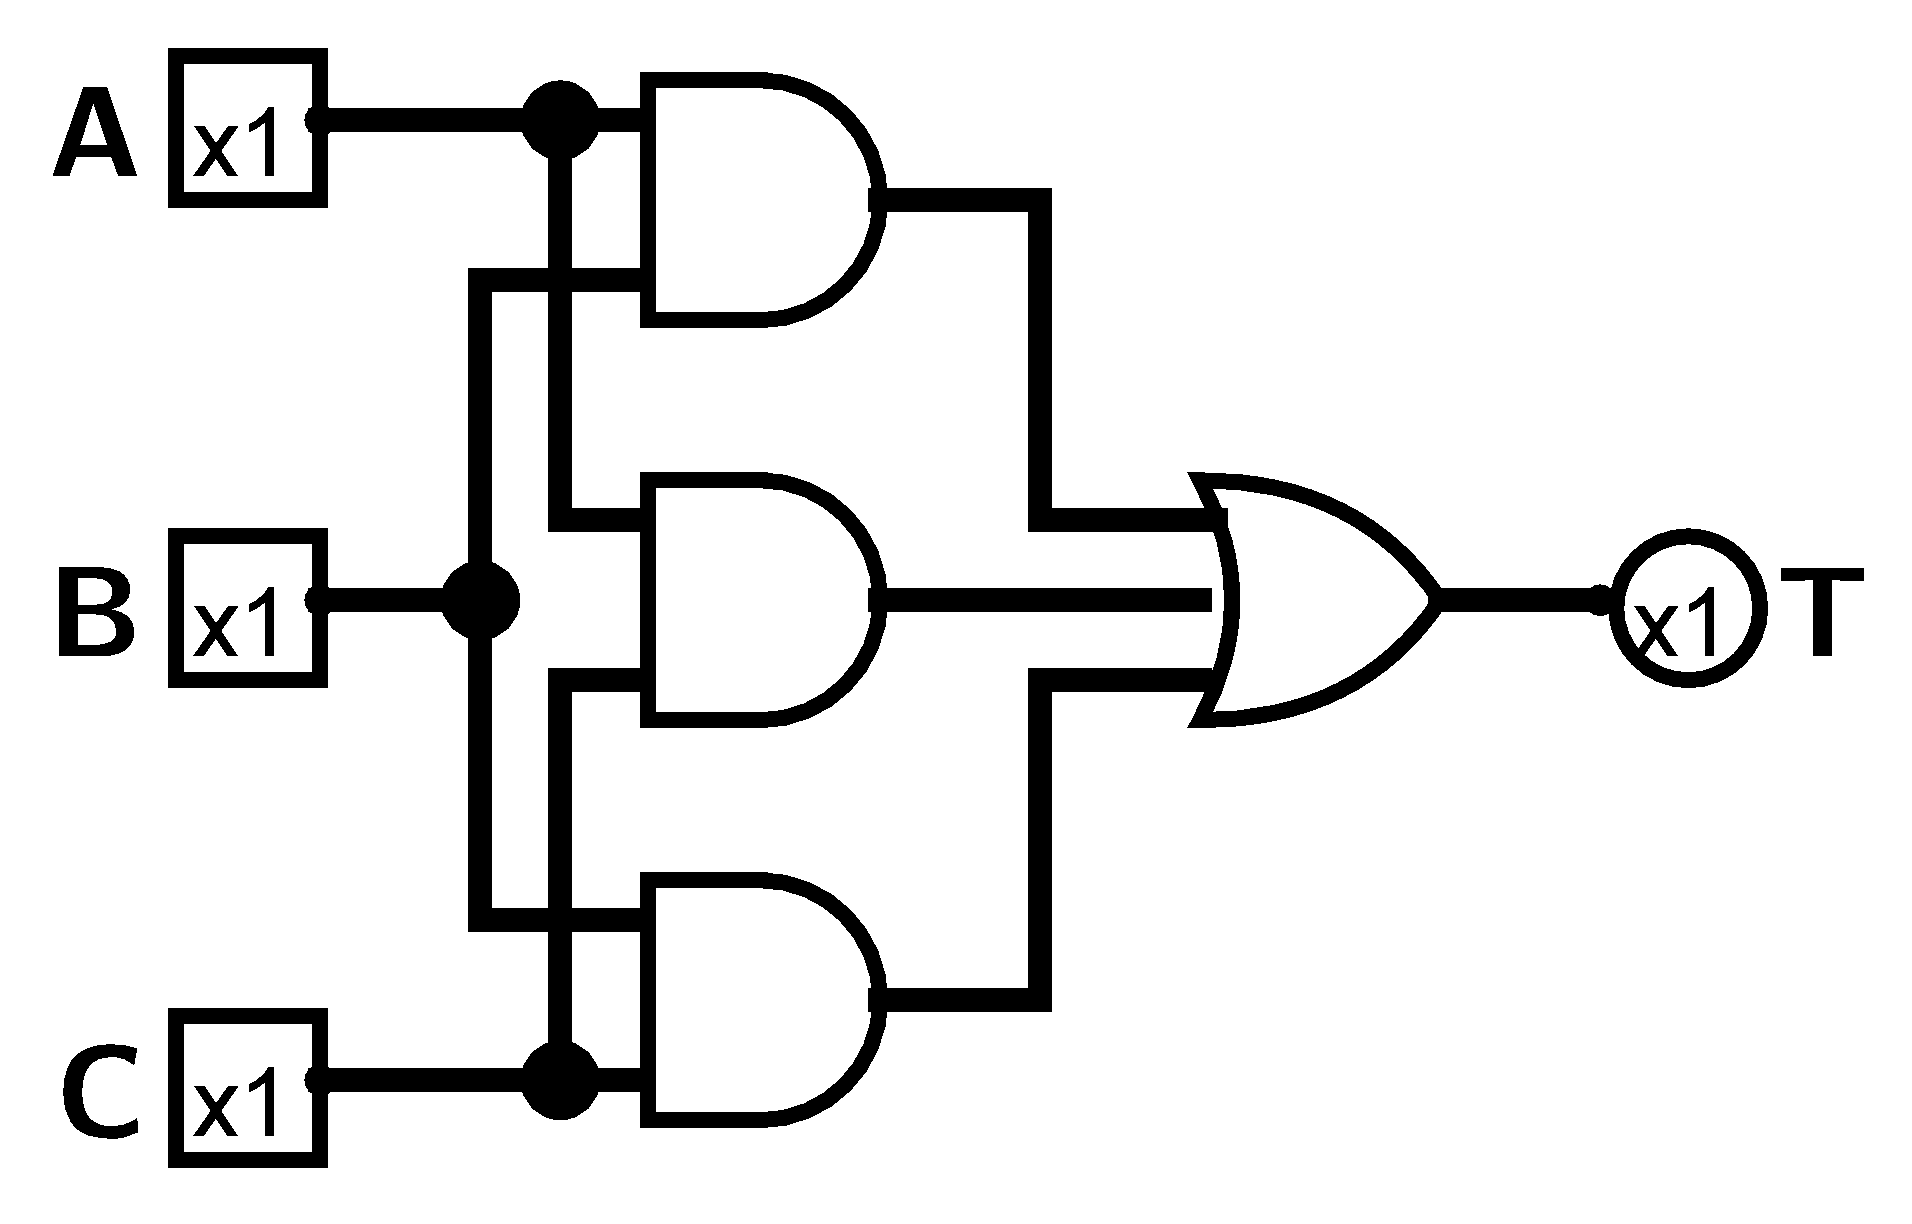
\includegraphics[width=0.6\textwidth]{Imagens/circ2a.png}
    \caption{Implementação da função $T$ apenas com AND e OR}
\end{figure}

\begin{figure}[H]
    \centering
    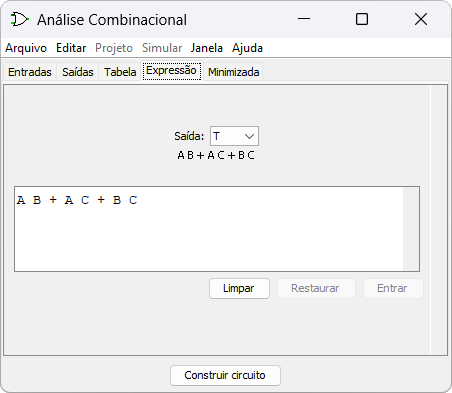
\includegraphics[width=0.4\textwidth]{Imagens/exprQ2a.png}
    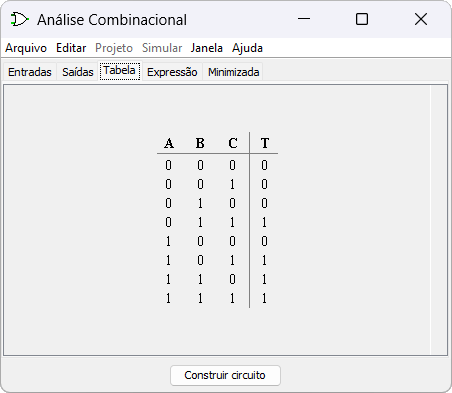
\includegraphics[width=0.4\textwidth]{Imagens/tabQ2a.png} \\
    \caption{Expressão e tabela-verdade gerados pelo Logisim para o circuito da figura 5}
\end{figure}

\subsection{Implementar a função S utilizando somente AND e OR}

\begin{figure}[H]
    \centering
    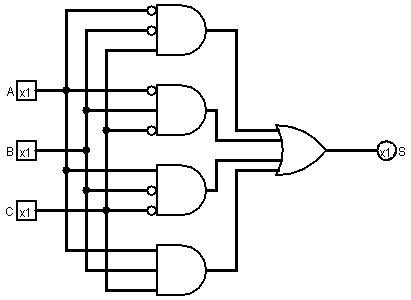
\includegraphics[width=0.6\textwidth]{Imagens/circ2b.png}
    \caption{Implementação da função $S$ apenas com AND e OR}
\end{figure}

\begin{figure}[H]
    \centering
    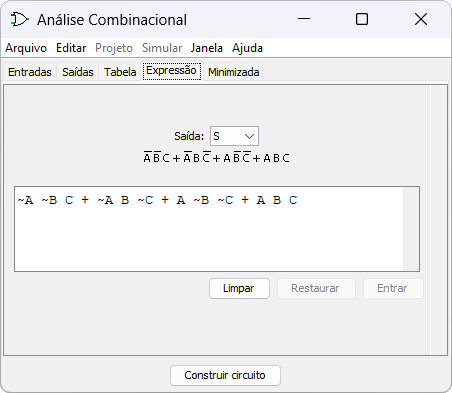
\includegraphics[width=0.4\textwidth]{Imagens/exprQ2b.png}
    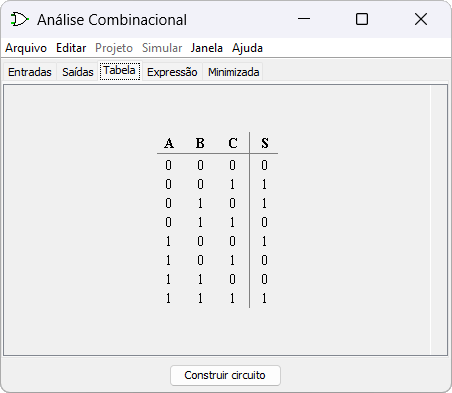
\includegraphics[width=0.4\textwidth]{Imagens/tabQ2b.png} \\
    \caption{Expressão e tabela-verdade gerados pelo Logisim para o circuito da figura 7}
\end{figure}

\section{Questão 3}
\paragraph{}
Nessa questão, considera-se as funções $T$ e $S$ do item anterior, porém, implementá-las-emos utilizando apenas a porta NAND.

\paragraph{}
Para entender o porquê de podermos implementar essas (e quaisquer outras) funções booleanas com a porta NAND, devemos primeiro conhecer o teorema da completude funcional de Sheffer.

\paragraph{Teorema da Completude Funcional de Sheffer:}
\textit{Dado um conjunto de operadores lógicos, diz-se que esse conjunto é funcionalmente completo se todas as funções booleanas podem ser expressas usando apenas esses operadores.}

\paragraph{}
O conjunto formado pelos operadores AND, OR e NOT, por exemplo, é completo funcional, i.e., qualquer função booleana pode ser implementada por essas três portas. Ainda mais incrível é que, como podemos implementar qualquer uma dessas portas apenas com a porta NAND - como está provado a seguir - concluímos que essa porta, sozinha, forma um conjunto funcionalmente completo (o mesmo é verdade para a porta NOR, mas isso não é relevante aqui).

\begin{table}[H]
    \centering
    \begin{tabular}{|>{\centering\arraybackslash}m{0.2\textwidth}|>{\centering\arraybackslash}m{0.6\textwidth}|}
        \hline
        Porta Lógica & Implementação com NAND \\ \hline
        NOT & 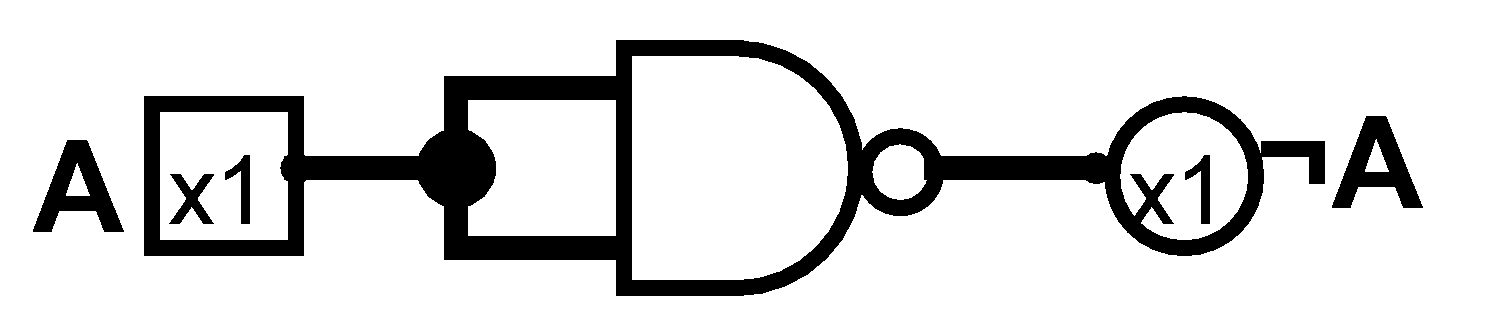
\includegraphics[width=0.4\textwidth]{Imagens/NOTcomNAND.png} \\ \hline
        AND & 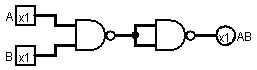
\includegraphics[width=0.4\textwidth]{Imagens/ANDcomNAND.png} \\ \hline
        OR & 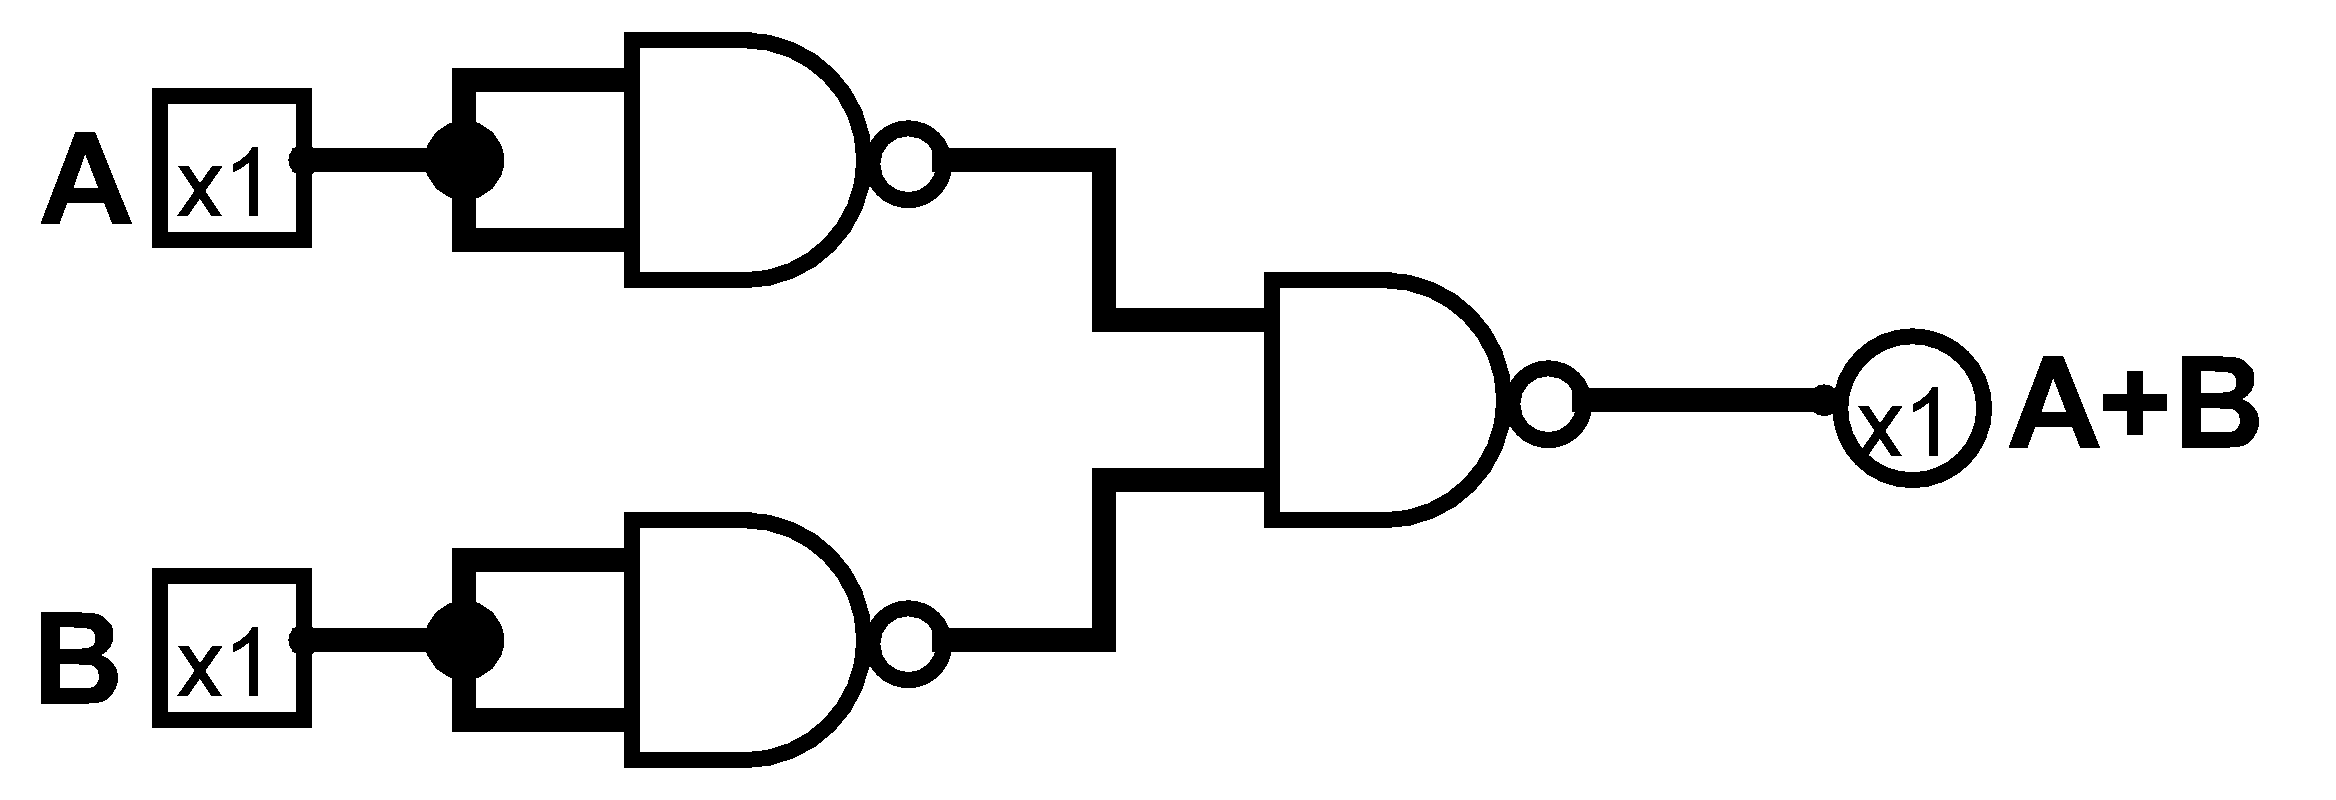
\includegraphics[width=0.4\textwidth]{Imagens/ORcomNAND.png} \\ \hline
    \end{tabular}
    \caption{Prova de que é possível implementar as portas AND, OR e NOT apenas com a porta NAND}
\end{table}

\paragraph{}
Note que uma forma de implementar as funções da questão 2 apenas com portas NAND é simplesmente substituir as portas AND, OR e NOT dos circuitos dessa questão pelas suas respectivas implementações com a porta NAND. A abordagem que faremos na presente questão, porém, é mais eficiente (utiliza menos portas lógicas): utilizaremos o primeiro teorema de De Morgan para manipular as expressões de cada função e chegar à sua implementação canônica com NANDs.

\paragraph{}
Provado que é possível implementar qualquer função booleana apenas com a porta NAND, resta a dúvida: por que fazer isso? A resposta está nas características físicas de cada porta lógica: a porta NAND é implementada com menos transistores do que as outras, por isso, é mais eficiente e barato produzir circuitos lógicos com essa porta.

\subsection{Implementar a função T utilizando somente NAND}
\paragraph{}
Para saber como implementar a função $T$ apenas com portas NAND, utilizaremos o primeiro teorema de De Morgan:

\[
T = AB + AC + BC = \overline{\overline{AB} \cdot \ \overline{AC} \cdot \ \overline{BC}},
\]
ou seja, $T$ é igual ao NAND entre os NANDs de $A$ e $B$, $A$ e $C$, $B$ e $C$. Precisamos somente aplicar essa lógica no Logisim e conseguimos montar o circuito abaixo.

\begin{figure}[H]
    \centering
    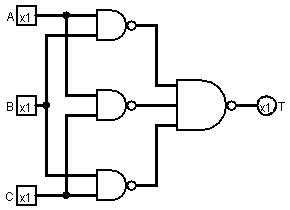
\includegraphics[width=0.5\textwidth]{Imagens/circ3a.png}
    \caption{Função $T$ implementada apenas com NANDs}
\end{figure}

\begin{figure}[H]
    \centering
    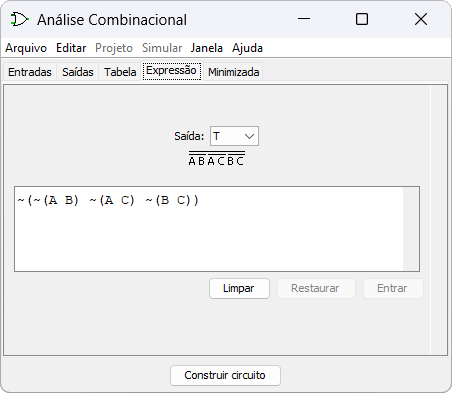
\includegraphics[width=0.4\textwidth]{Imagens/exprQ3a.png}
    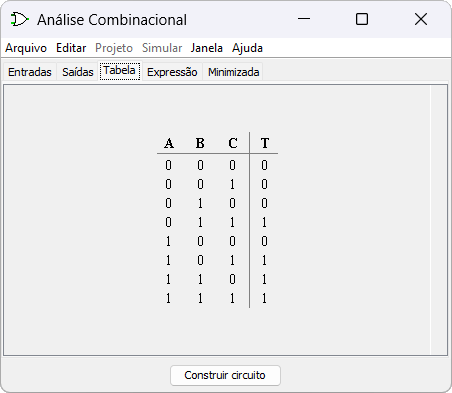
\includegraphics[width=0.4\textwidth]{Imagens/tabQ3a.png} \\
    \caption{Expressão e tabela-verdade gerados pelo Logisim para o circuito da figura 9}
\end{figure}

\subsection{Implementar a função S utilizando somente NAND}
\paragraph{}
Para saber como implementar a função $S$ apenas com portas NAND, utilizaremos, novamente, o primeiro teorema de De Morgan:

\[
S = \overline{A} \ \overline{B} \ C + \overline{A} \ B \ \overline{C} + A \ \overline{B} \ \overline{C} + A \ B \ C = \overline{\overline{\overline{A} \ \overline{B} \ C} \cdot \overline{\overline{A} \ B \ \overline{C}} \cdot \overline{A \ \overline{B} \ \overline{C}} \cdot \overline{A \ B \ C}}
\]
ou seja, $S$ é igual ao NAND entre os NANDs de $\overline{A}$, $\overline{B}$ e $C$; $\overline{A}$, $B$ e $\overline{C}$; $A$, $\overline{B}$ e $\overline{C}$; $A$, $B$, $C$. Novamente, precisamos somente aplicar essa lógica no Logisim e montamos o circuito a seguir.

\begin{figure}[H]
    \centering
    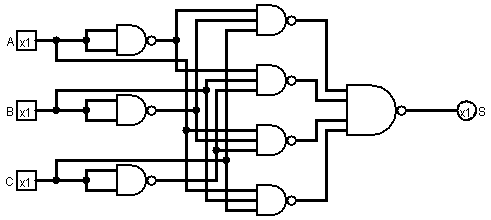
\includegraphics[width=0.6\textwidth]{Imagens/circ3b.png}
    \caption{Função $S$ implementada apenas com NANDs}
\end{figure}

Podemos deixar esse circuito um pouco mais bonito tratando as inversoras como caixas-pretas:

\begin{figure}[H]
    \centering
    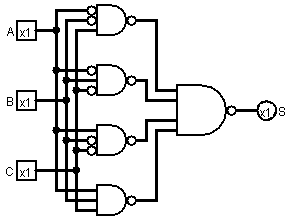
\includegraphics[width=0.6\textwidth]{Imagens/circ3b2.png}
    \caption{Função $S$ simplificada implementadas com NANDs}
\end{figure}

\begin{figure}[H]
    \centering
    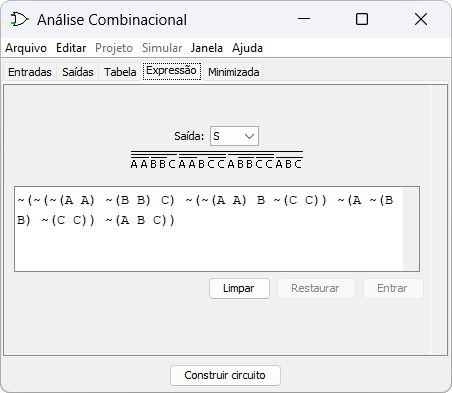
\includegraphics[width=0.4\textwidth]{Imagens/exprQ3b.png}
    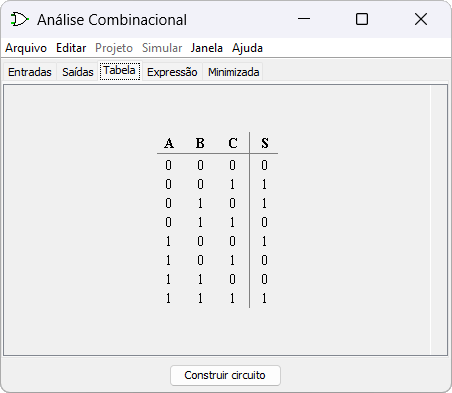
\includegraphics[width=0.4\textwidth]{Imagens/tabQ3b.png} \\
    \caption{Expressão e tabela-verdade gerados pelo Logisim para o circuito da figura 11}
\end{figure}

\section{Questão 4}
\paragraph{}
Um multiplexador é um dispositivo digital que, dadas $n$ entradas de dados ($D$), seleciona como saída uma delas por meio das suas $\log_2n$ entradas de seleção ($S$). Nessa questão, implementamos o circuito lógico de um multiplexador 4-para-1, i.e., o multiplexador com 4 entradas de dados, modelado pela expressão
\[
Y = D_0 \ \overline{S_1} \ \overline{S_0} + D_1 \ \overline{S_1} \ S_0 + D_2 \ S_1 \ \overline{S_0} + D_3 \ S_1 \ S_0.
\]
A tabela-verdade desse dispositivo é a que segue.

\begin{table}[H]
    \centering
    \begin{tabular}{|c|c|c|}
        \hline
        \rowcolor{black}
        \textcolor{white}{$S_1$} & \textcolor{white}{$S_0$} & \textcolor{white}{$Y$} \\ \hline
        0 & 0 & $D_0$ \\ \hline
        \rowcolor{lightgray}
        0 & 1 & $D_1$ \\ \hline
        1 & 0 & $D_2$ \\ \hline
        \rowcolor{lightgray}
        1 & 1 & $D_3$ \\ \hline
    \end{tabular}
    \caption{Tabela-verdade multiplexador 4x1}
\end{table}

\paragraph{}
Como devemos implementar $Y$ apenas com NANDs, precisamos, novamente, usar De Morgan para chegar à expressão que nos fornece a implementação diretamente.

\[
Y = D_0 \ \overline{S_1} \ \overline{S_0} + D_1 \ \overline{S_1} \ S_0 + D_2 \ S_1 \ \overline{S_0} + D_3 \ S_1 \ S_0
\]
\[
\Rightarrow Y = \overline{\overline{D_0 \ \overline{S_1} \ \overline{S_0}} \cdot \overline{D_1 \ \overline{S_1} \ S_0} \cdot \overline{D_2 \ S_1 \ \overline{S_0}} \cdot \overline{D_3 \ S_1 \ S_0}}.
\]
O circuito que implementa essa função é o que segue:

\begin{figure}[H]
    \centering
    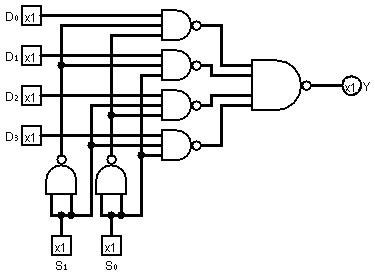
\includegraphics[width=0.7\textwidth]{Imagens/circ4.png}
    \caption{Implemetação da função $Y$ apenas com NANDs}
\end{figure}

\paragraph{}
Novamente, para melhorar a visualização, podemos simplificar a implementação tratando as inversoras como caixas pretas. Essa implementação está apresentada abaixo.

\begin{figure}[H]
    \centering
    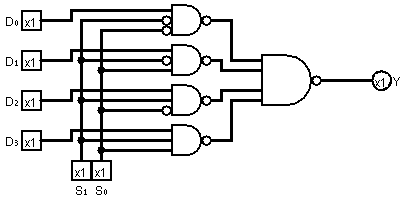
\includegraphics[width=0.7\textwidth]{Imagens/circ4_2.png}
    \caption{Implemetação da função $Y$ simplificada}
\end{figure}

\begin{figure}[H]
    \centering
    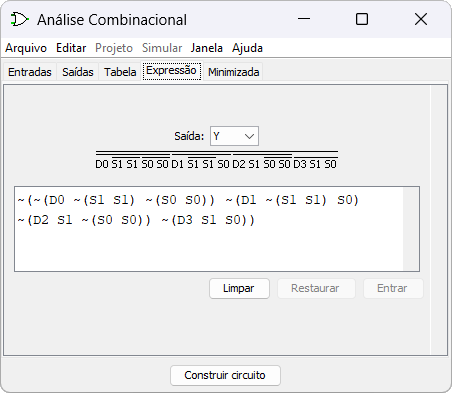
\includegraphics[width=0.8\textwidth]{Imagens/exprQ4.png}
    \caption{Expressão gerada pelo Logisim para o circuito da figura 14}
\end{figure}

\begin{figure}[H]
    \centering
    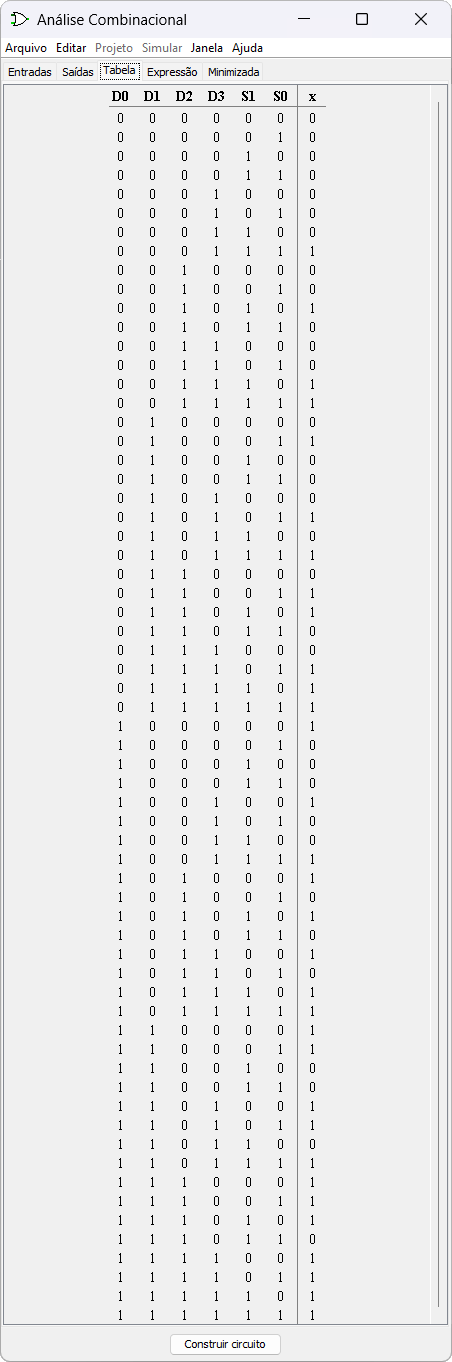
\includegraphics[width=0.5\textwidth]{Imagens/tabQ4.png}
    \caption{Tabela-verdade gerada pelo Logisim para o circuito da figura 14}
\end{figure}

\end{document}